\section{Experiments}\label{dmp:experiments}

\begin{table}[t]
\centering
\footnotesize
\tabcolsep=0.11cm
\begin{tabular}{|l|c|c|c||c|c|}
\hline
& Surface & Contour & Implicit & RIMLS\cite{rimls} & SPSR\cite{spsr} \\
\hline
bunny & \textbf{2.71E-04} & 6.64E-04 & 5.52E-04 & 1.43E-03 & 3.96E-04 \\
dragon & \textbf{4.18E-04} & 6.12E-04 & 1.20E-03 & 1.65E-03 & 1.46E-02 \\
car & \textbf{2.73E-04} & 4.57E-04 & 6.83E-02 & 1.50E-03 & 2.10E-03 \\
cup &  \textbf{2.59E-04} & 5.80E-04 & 2.64E-02 & 1.74E-03 & 1.00E-02 \\
mobius &  \textbf{3.51E-04} & 4.95E-04 & 3.26E-03 & 1.96E-03 & 1.89E-02 \\
chair &  \textbf{3.95E-04} & 4.22E-04 & 7.32E-03 & 2.09E-03 & 2.58E-02 \\
spiral &  1.05E-03 & \textbf{7.31E-04} & 1.64E-02 & 2.98E-03 & 7.90E-02 \\
ring &  5.69E-04 & \textbf{5.54E-04}& 4.81E-02 & 2.46E-03 & 3.76E-02 \\
\hline
avg. & \textbf{4.48E-04} & 5.65E-04& 2.13E-02 & 1.98E-03 & 2.36E-02 \\
\hline
\end{tabular}
\vspace{4pt}
\caption{ \small \label{tab:denoising} \textbf{Quantitative results for point cloud denoising.}
\emph{Surface}, \emph{Contour} and \emph{Implicit} represent different \emph{deep manifold priors} based on a 2-manifold, 1-manifold and level-set paramertization.
}
\vspace{-15pt}
\end{table}
\begin{table*}[t]
\centering
\scriptsize
\tabcolsep=0.11cm
\begin{tabular}{|l|c|c|c|c||c|c|}
\hline
& S1R & S8R & S1 & S8 & - & - \\
\hline
avg. & 4.48E-03 & \textbf{4.48E-04} & 2.75E-03 & 1.35E-03  & - & - \\
\hline \hline
& C1R & C8R & C1 & C8 & RIMLS\cite{rimls} & SPSR\cite{spsr} \\
\hline
avg. & 1.08E-03 & 5.77E-04 & 1.00E-03 & 5.82E-04 & 1.98E-03 & 2.36E-02 \\
\hline
\end{tabular}
\vspace{4pt}
\caption{ \small \label{tab:ablation} \textbf{Ablation studies.}
Comparison between different variations of our approach.
Naming follows the following convention: S corresponds to a 2-manifold parameterization (surface), whereas C corresponds to a 1-manifold (contour).
The following number (1 or 8) corresponds to the number of parameterizations.
A R letter is added if stretch regularization was used ($\lambda=1.0$).
}
\end{table*}

\begin{figure*}[t]
\centering
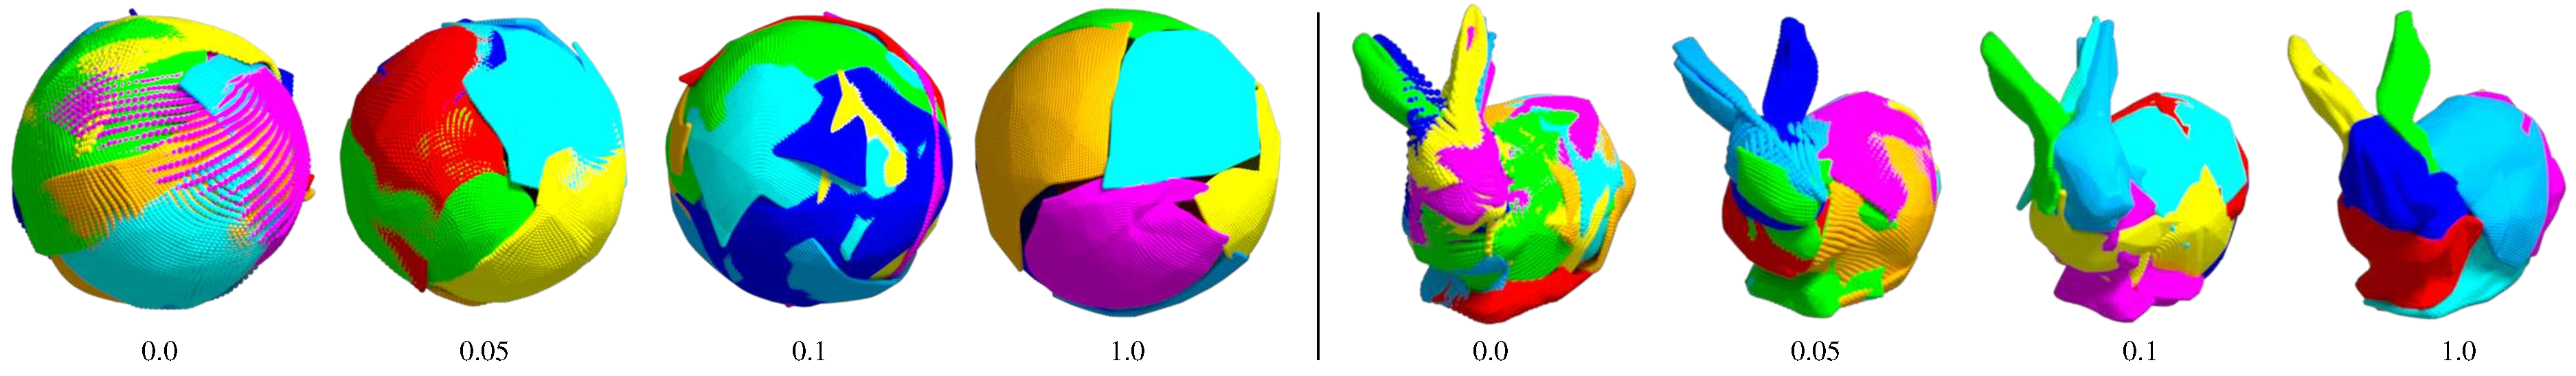
\includegraphics[width=\linewidth]{dmp/imgs/regularization.pdf}
	\caption{\label{fig:reg} \small
	\textbf{Effect of the regularization weight on the reconstructed manifold.} 
	For this experiment, we use our method to reconstruct a sphere using an atlas with 8 charts and render each one with a different color.
	Without any regularization, there is a significant amount of deformation applied to each surface (hence the space between the points) and a considerable amount of overlap between different parts. As the regularization weight increases, those aspects are
	noticeably reduced. 
	\small}
	\vspace{-12pt}
\end{figure*}

In this section we will present quantitative and qualitative results for
applying the manifold prior to multiple manifold reconstruction tasks.
All the experiments in this paper were implemented using Python 3.6 and PyTorch.
Computation was performed on TitanX GPUs. 

\subsection{Denoising and Interpolation}

\paragraph*{Benchmark} Our benchmark consists of 8 different 3D shapes with diverse characteristics.
The shapes are normalized to fit a unit cube and 16K points are sampled on their surfaces.
The point positions are perturbed by a Gaussian noise with standard deviation $2\times10^{-3}$ and zero mean.
Figure~\ref{fig:denoising} shows the ground-truth shapes as well
as their noisy counterpart.
Since the level-set representation and the baseline methods 
(RIMLS~\cite{rimls},  SPSR~\cite{spsr}) 
require normal information, we estimate the normal for every point by using the local frame defined by its nearest neighbors.
We experimented multiple numbers of neighbors for both baselines and used the value that led to the best results: 20 neighbors for SPSR and the level-set representation, 30 neighbors for RIMLS.
The network used in the level-set representation follows the same architecture
and training protocol
as the one used for the explicit parametrizations (described in the next paragraph).
However, it is trained to predict every point as outside (+1) or inside the surface (-1).
Points with positive values are generated by translating every point in the point cloud along the normal direction for a distance $\epsilon=2\times10^{-3}$.
Points with negative values are generated in the same way, but applying a displacement
to the opposite direction.
For RIMLS, we used a relative spatial filter size of 10, 15 projection iterations and a volumetric grid with $200^3$ resolution.
For SPSR, we used an octree with depth 7 and 8 iterations.

\paragraph*{Experimental setup}
Our method performs denoising by minimizing Equation~\ref{eq:objective}.
In this framework, $P$ is the noisy point cloud we are trying to reconstruct and $\bm{f_\theta}$ is a neural network.
In all experiments we use a neural network with 3 fully connected layers,
where the layers have 256, 128 and 64 hidden units, respectively.
The output of the networks is a point in $\mathbb{R}^3$.
The input can be either a point in $\mathbb{R}$ (1-manifold) or $\mathbb{R}^2$ (2-manifold).
We use $ReLU$ activations followed by batch normalization at each layer, except for the last, where we use a $tanh$ non-linearity.
We vary the architecture of $\bm{f_\theta}$ with respect to the number
of parameterizations (1 or 8) and dimensionality (1 or 2).
Additionally, we try each one of these architectural variations with
$\lambda=0$ and $\lambda=1.0$.
When using 8 parametrizations, 4096 points are sampled per parametrization.
When using just one parametrization, 16K points are sampled.
We optimize our objective through gradient descent using the Adam optimizer
with learning rate $10^{-3}$.
For evaluation, we uniformly sampled 16K points in the computed manifold (represented as a triangular mesh) and compute the Chamfer distance with respect to the ground-truth.

\paragraph*{Results and discussion.}
Our methods significantly outperform the baselines for most of the shapes.
Quantitative results can be seen in Table~\ref{tab:denoising} and the qualitative results are shown in Figure~\ref{fig:denoising}.
The numbers are computed using 8 parametrizations (for surfaces and curves) and
$\lambda=1.0$.
A comparison between different variations of our approach is displayed in Table~\ref{tab:ablation}.
RIMLS, SPSR and level-set representations (\emph{Implicit} in Table~\ref{tab:denoising}) 
have trouble reconstructing point clouds with a significant amount of noise.
This is due to the fact that those methods rely on accurate surface normal estimates to infer
inside/outside regions of the shape.
Besides, RIMLS and methods based on implicit functions (SPSR and level-set representations) work better when dealing with closed surfaces. 
Shapes that are better approximated by contours (ring, spiral, chair's legs) are particularly challenging for those approaches.
On the other hand, the networks parametrizing explicit functions (\emph{Surface} and \emph{Contour} in Table~\ref{tab:denoising}) are able to adapt to different structures and
present a fair performance across a diverse set of shapes.

The results in Table~\ref{tab:ablation} suggest that using multiple parametrizations gives a better approximation than just using a single one.
This happens because complex shapes are easier to represent by multiple parametrizations.
For example, while using a single 2-manifold parametrization, the ring tends to be approximated by a disk, which significantly increases the reconstruction error when
the points are uniformly sampled over the final mesh.
This behavior is illustrated in Figure~\ref{dmp:interp}.
Our ablation studies also indicate that using stretch regularization helps
parametrizations of both surfaces and contours.
Figure~\ref{fig:reg} shows the effect of stretch regularization for
two different shapes.
As the regularization weight increases, the overlap between different parameterizations becomes smaller.
When overlaps exist, the manifold representation is suboptimal --
the same regions are being generated multiple times.

\begin{figure}
\centering
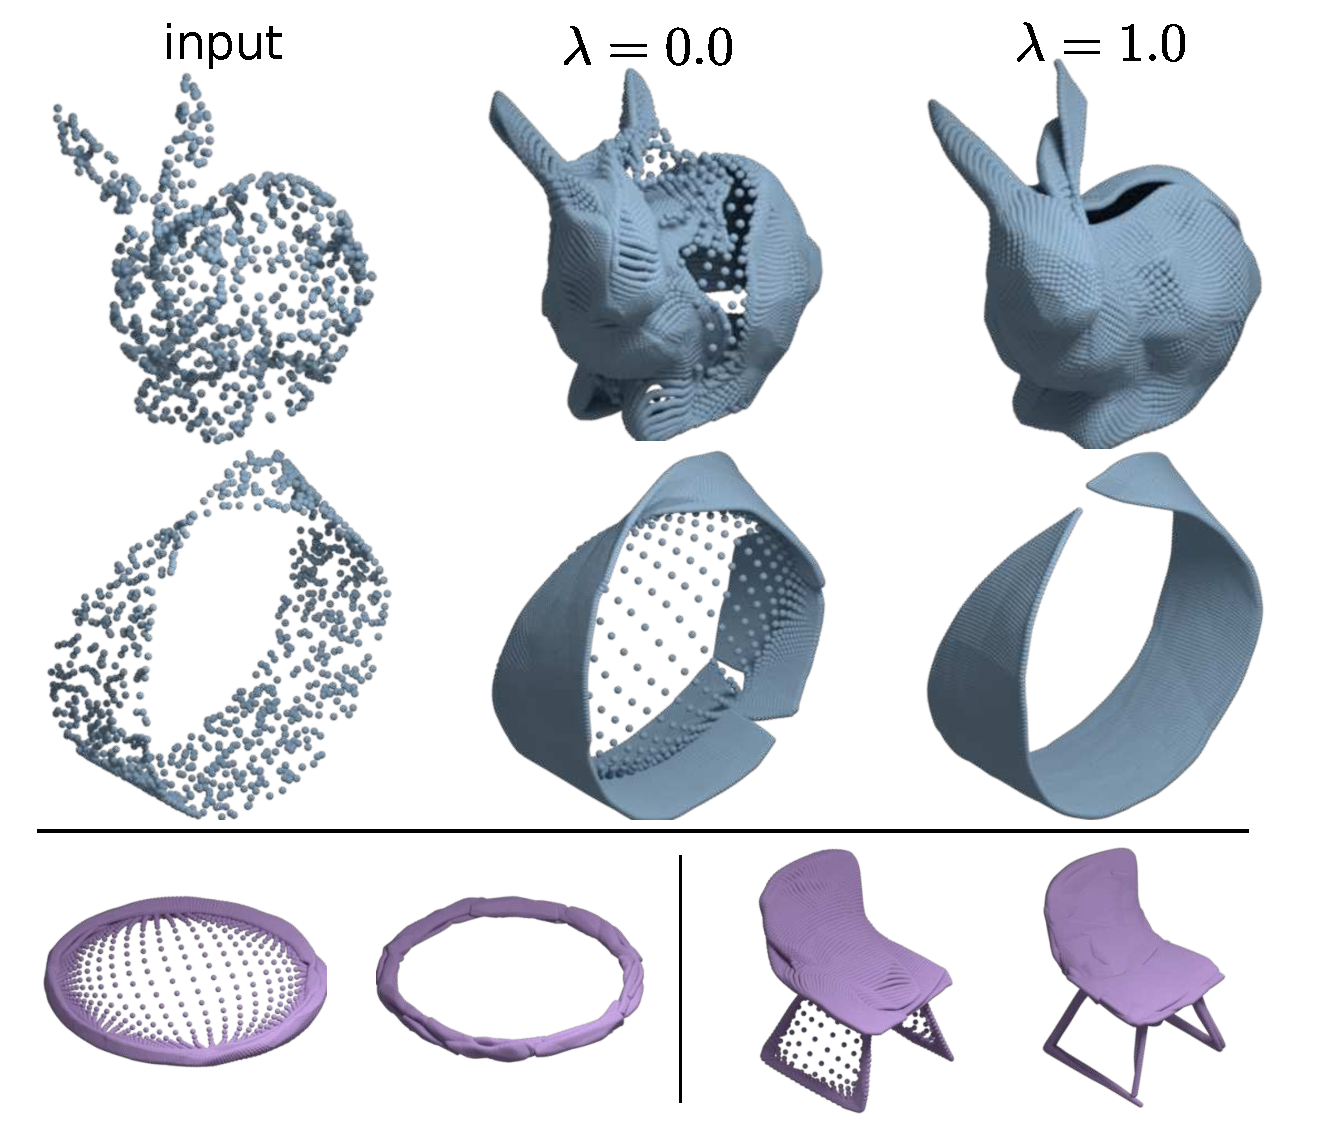
\includegraphics[width=0.6\linewidth]{dmp/imgs/interp_rings.pdf}
    \caption{\label{dmp:interp} \small 
    \emph{Interpolation results on the top.}
    Stretch regularization ($\lambda=1.0$) helps
    generate smoother surfaces.
    \emph{On the bottom, denoising using one vs. multiple parametrizations.}
   Shapes on the left were reconstructed using a single parameterization, 
    whereas shapes on the right used 8 parameterizations. 
    Using multiple parameterizations helps reconstruct complex shapes.
}
\vspace{-10pt}
\end{figure}


\begin{figure}[t!]
\centering
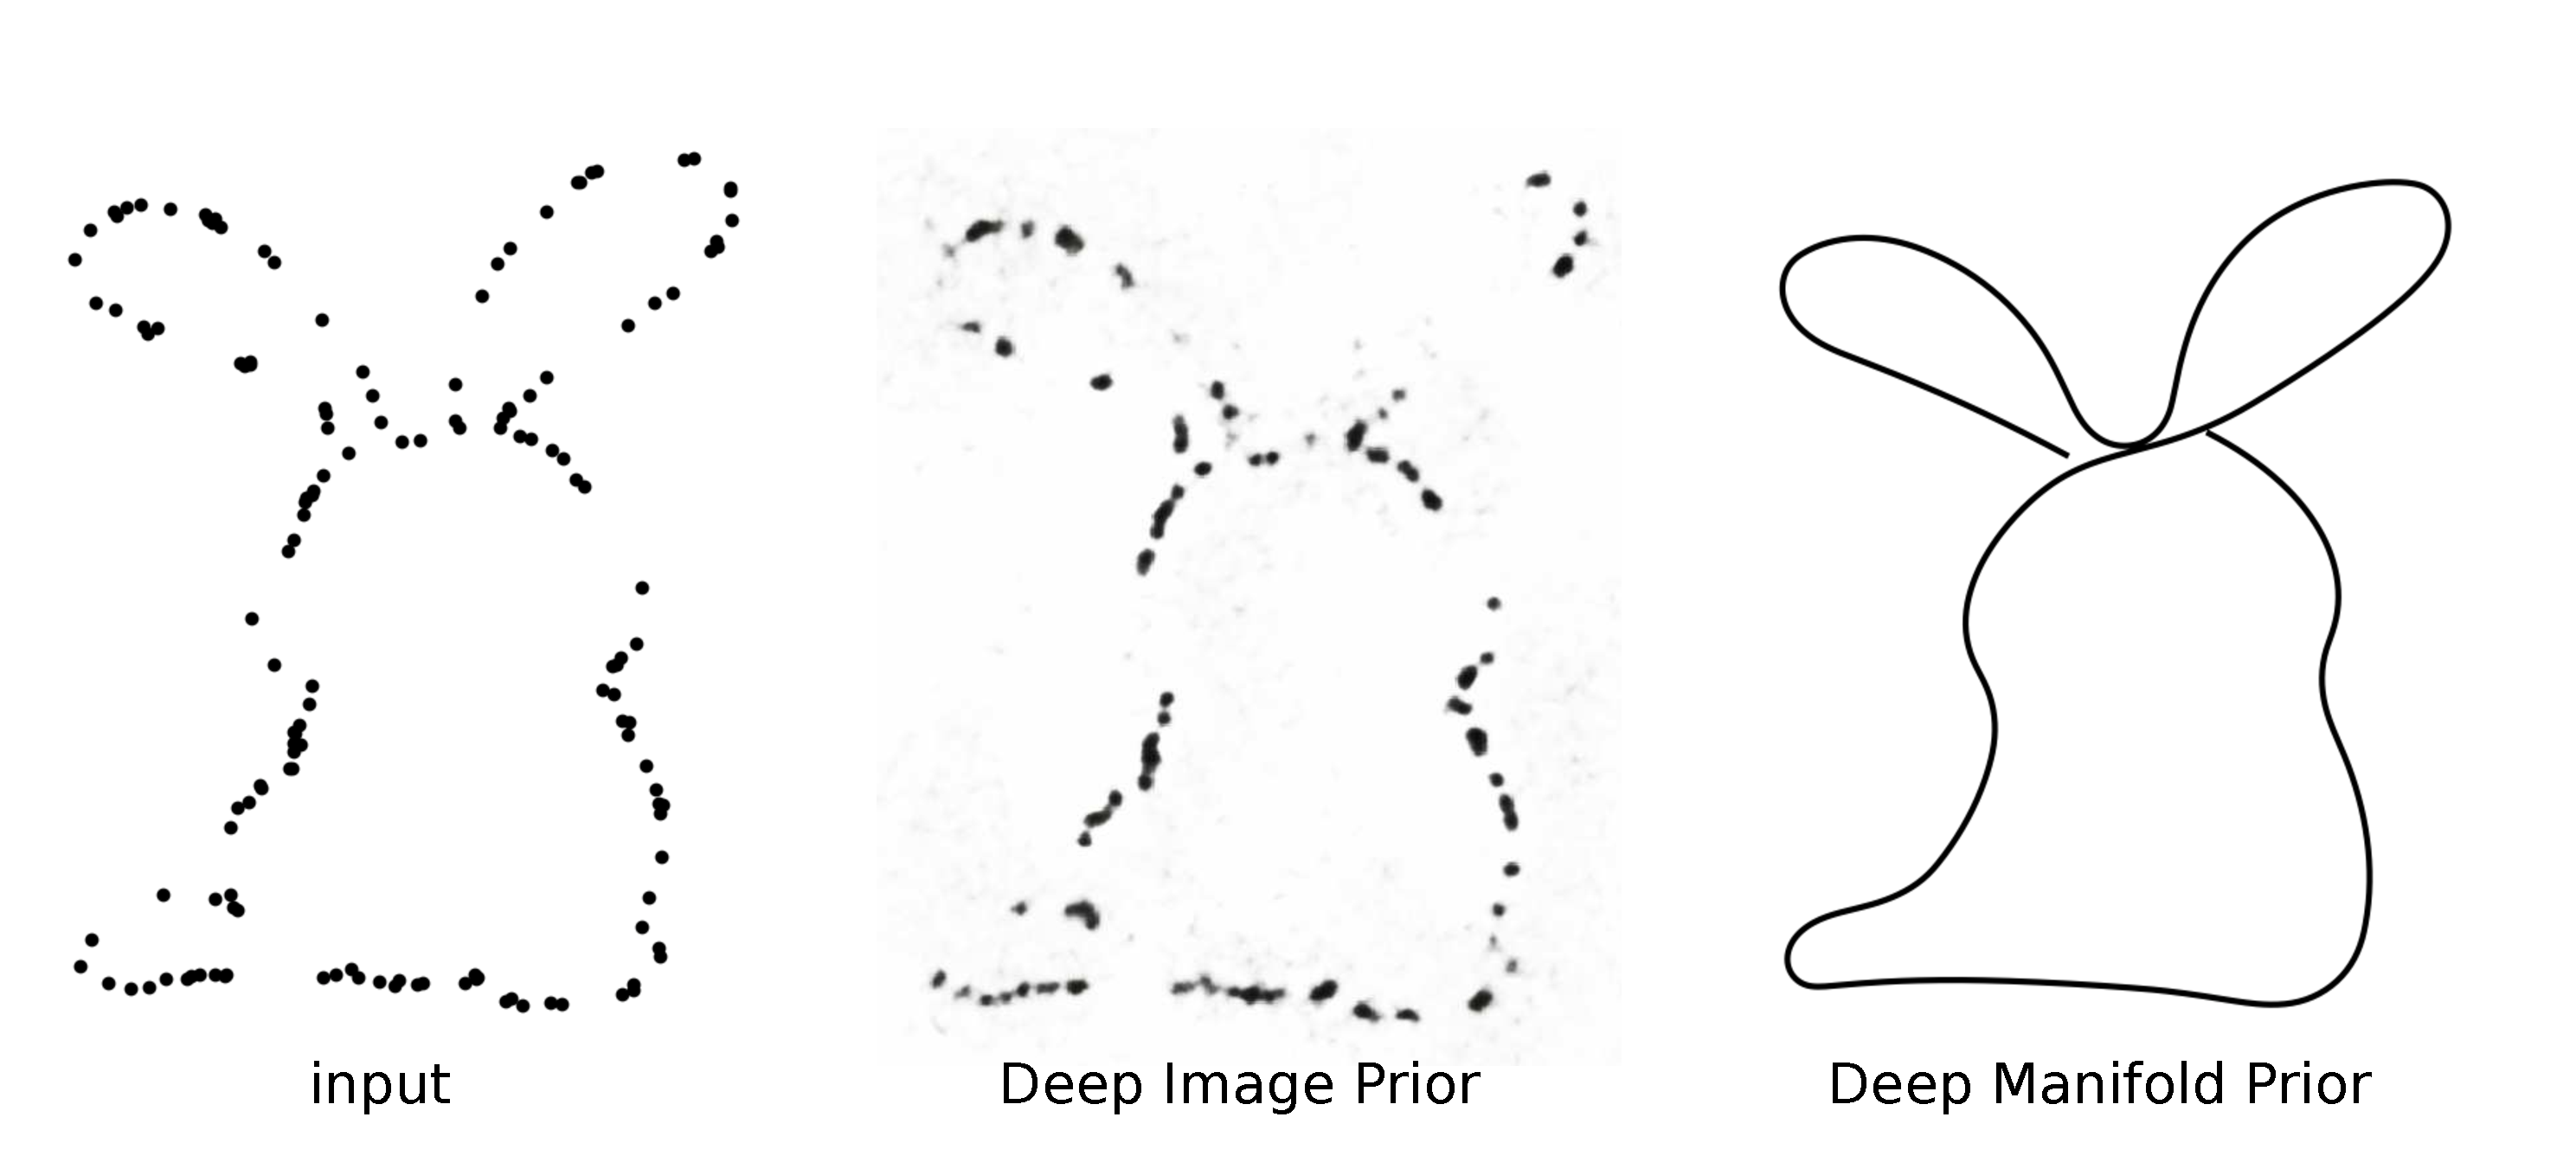
\includegraphics[width=0.8\linewidth]{dmp/imgs/dipcomp.pdf}
	\caption{\label{fig:dipcomp} \small
	\textbf{Comparison to the deep image prior~\cite{dip}.}
	Image-based prior (middle) is not able to connect the dots in the input image (left).
	On the other hand, the manifold prior is able to reasonably interpolate the dotted
	drawing.
	}
	\vspace{-18pt}
\end{figure}


\begin{figure*}[t]
\centering
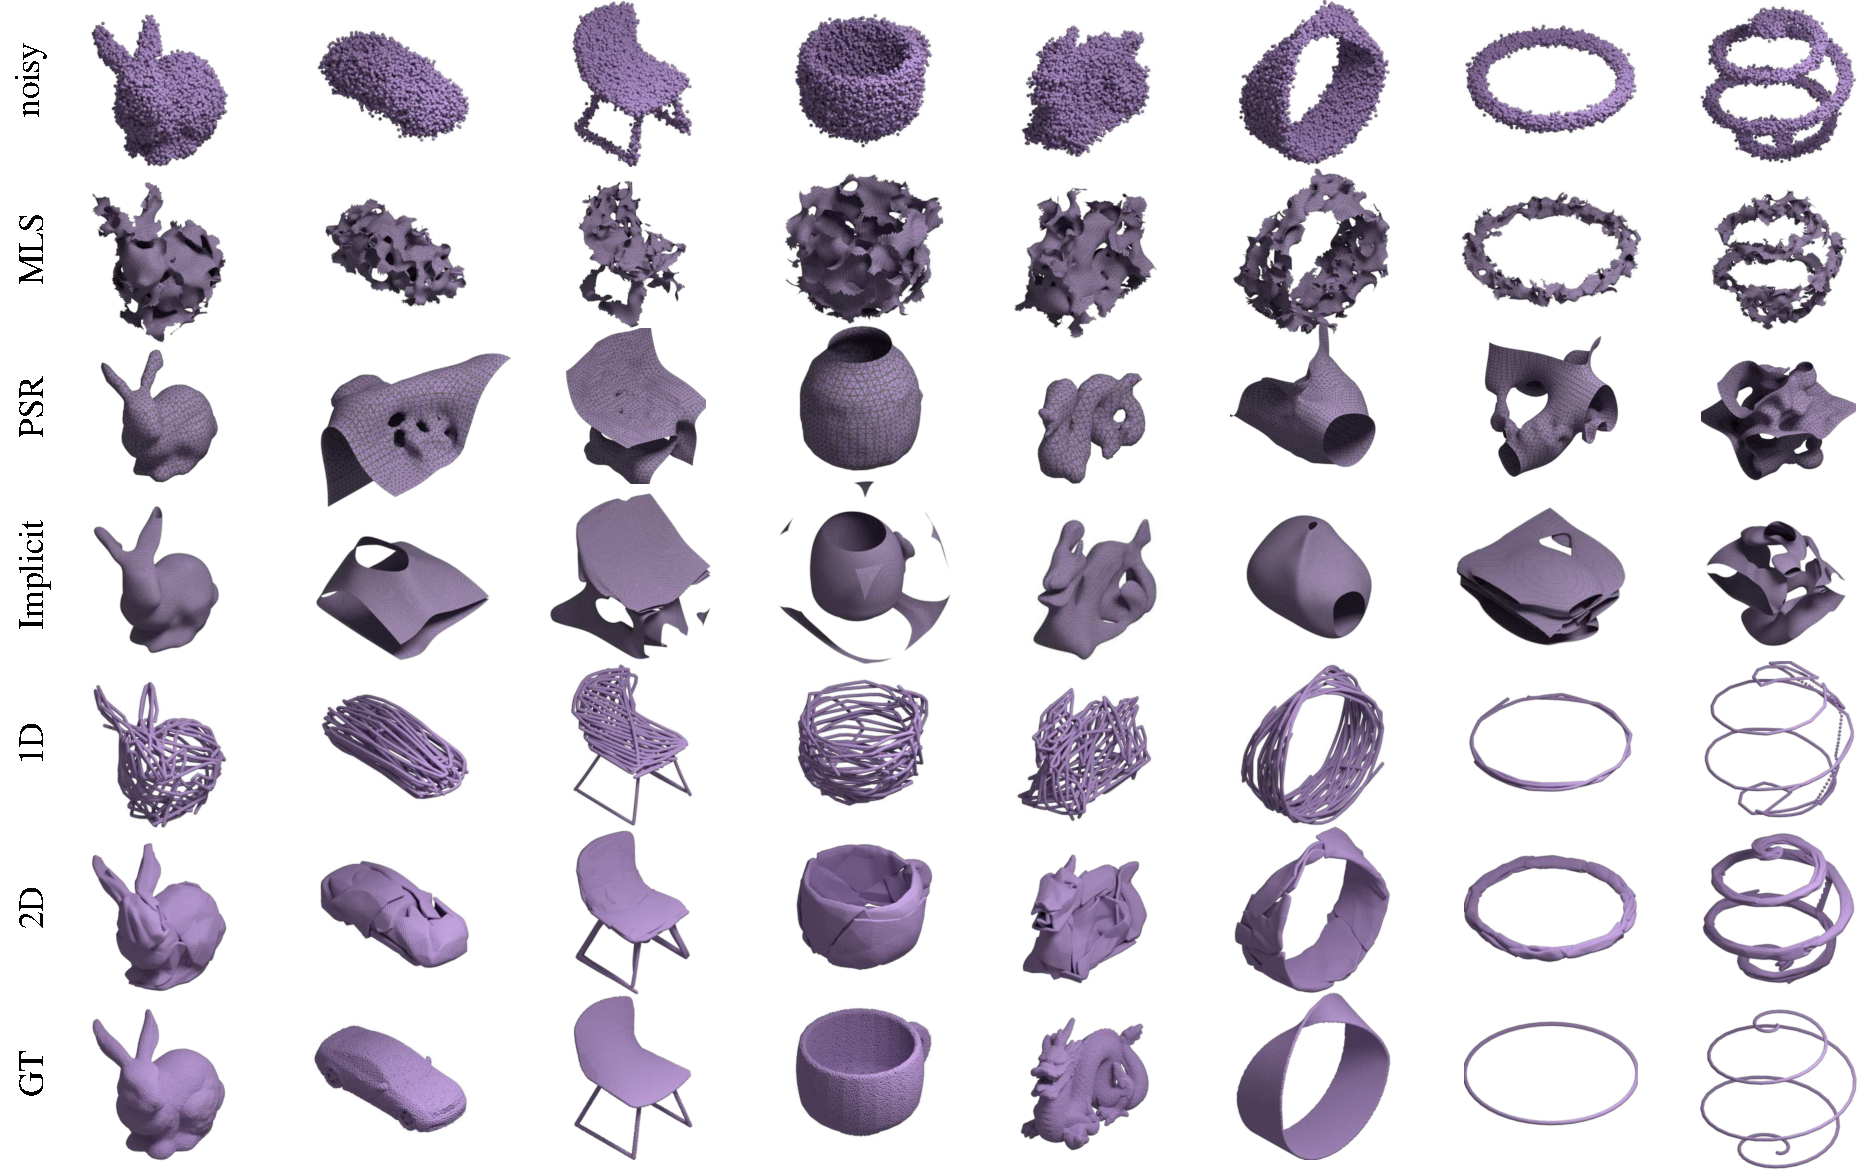
\includegraphics[width=1.0\linewidth]{dmp/imgs/denoising.pdf}
	\caption{\label{fig:denoising} \small
	\textbf{Qualitative comparison between different denoising methods.}
	Rows display different methods, whereas columns display different shapes.
	Baseline methods do not perform as well as the deep manifold prior, even for closed surfaces like the bunny (first column) and the dragon (fifth column).
	As we can see, 2-manifold parameterizations are better for reconstructing surfaces, whereas 1-manifold counterparts reconstruct the curves (last two columns) more
	acurattely.
	\small}
\end{figure*}

\paragraph*{Interpolation} We also explored using the manifold prior for point cloud interpolation.
This experiment follows the same experimental setup as denoising.
However, instead of perturbing the points with Gaussian noise, we randomly select 1K points out of 16K.
Interpolation is performed by minimizing Equation~\ref{eq:objective}.
Results can be seen in Figure~\ref{dmp:interp}.
For these experiments we use a single parameterization and include stretch regularization, without which the surface has holes and significant folds.
Our method is able to reconstruct reasonable surfaces from a small
set of points.

\paragraph*{Comparison with the deep image prior}
We also compare our approach to the deep image prior~\cite{dip} for interpolating points in 2D
images.
Results are presented in Figure~\ref{fig:dipcomp}.
We use the same architecture from \cite{dip} while minimizing
the mean squared error with respect to the image pixels.
For the manifold prior, we use a single 1-manifold parameterization following
the architecture described before, differing only in the dimensionality of the output: points this this case are in $\mathbb{R}^2$ instead of $\mathbb{R}^3$.
Coordinates of the black pixels in the input image are used to form a point cloud and 
the manifold is computed by minimizing Chamfer distance with respect to it.

\begin{figure}
\centering
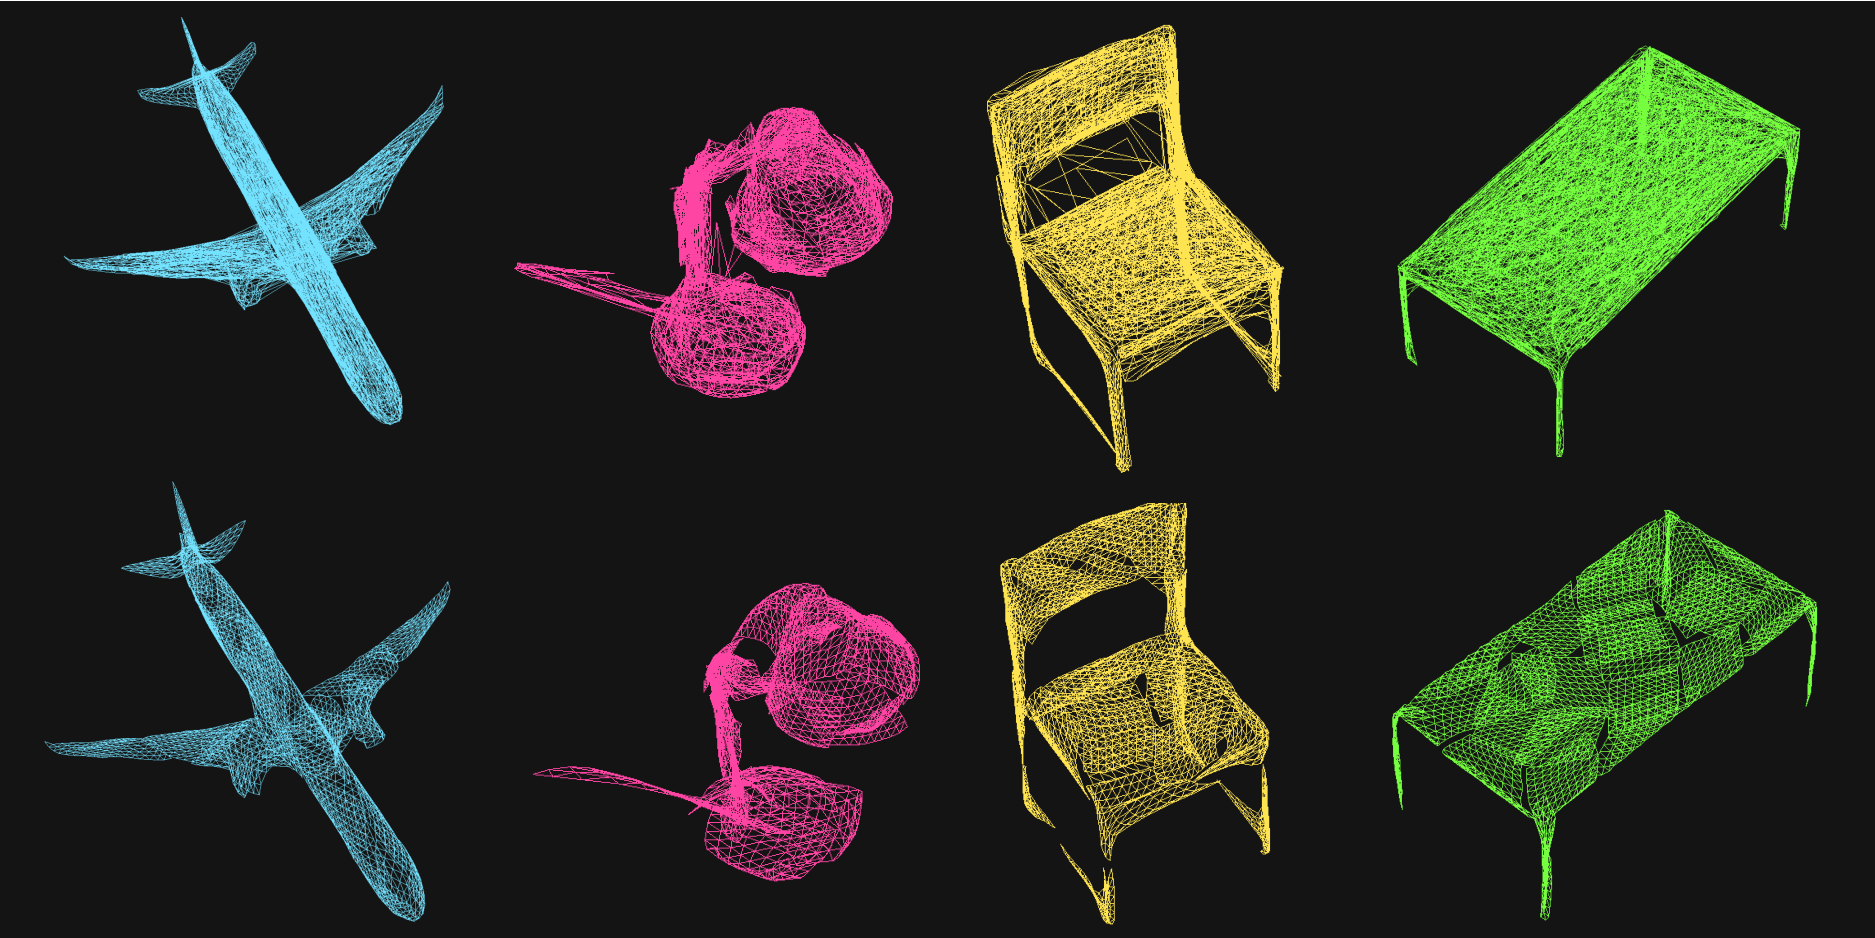
\includegraphics[width=0.8\linewidth]{dmp/imgs/aestretch.pdf}
    \caption{\label{fig:aestretch} \small \textbf{Autoencoder results}.
    Results on using AtlasNet~\cite{atlasnet} trained w/o (top) and w/ (bottom) stretch regularization.
    The latter results in meshes with reduced deformation and overlap, and removes artifacts where the chair's back is incorrectly filled.
}
\end{figure}

\subsection{Learning from data}\label{sec:exp_data}
Finally, we show how the insights presented in the earlier sections, in particular convolutional parameterization and stretch regularization, can also improve generative models of 3D shapes when trained on a large collection of shapes. 

To measure the effect of the stretch regularization in a learning-based scenario,
we train a model using the same architecture as AtlasNet~\cite{atlasnet} on a subset of $50,000$ shapes across $13$ categories of the ShapeNet dataset~\cite{chang2015shapenet}.
Adding stretch regularization did not significantly impact the Chamfer metric -- error of $1.46 \times 10^{-3}$ and $1.47 \times 10^{-3}$ with and without regularization.
However, the results are qualitatively better. 
As seen in Figure~\ref{fig:aestretch} the regularization reduces the stretch and overlap of the generated surfaces, and eliminates artifacts where holes are incorrectly filled.

We also train a convolutional decoder with stretch regularization on the single-view reconstruction benchmark~\cite{choy20163d}.
Our approach called ConvAtlas is compared against AtlasNet and MRTNet~\cite{mrt18} in Table~\ref{tab:svr}.
For a fair comparison, we use 4K points for evaluation across all methods.
ConvAtlas outperforms both approaches in terms of per-category and per-instance error, and also leads to more compact models.
Per-category results and experimental details are in the Supplementary material.


\begin{table}[t!]
\tabcolsep=0.11cm
\centering
\small
\begin{tabular}{|l|c|c|c|}
    \hline
    Architecture &  mean/cat. & mean/inst. & \#params. \\
    \hline
    MRTNet & 4.80 & 4.26 & 81.6M\\
    AtlasNet & 4.74 & 4.38 & 42.6M\\
    ConvAtlas & \textbf{4.53} & \textbf{4.00} & \textbf{ 14.5M}\\
    \hline
\end{tabular}
\vspace{4pt}
\caption{\small \textbf{Quantitative results for single-view image-to-shape reconstruction.} The table reports the mean Chamfer distance metric (scaled by $10^3$) computed per category and per instance.
  }
  \label{tab:svr}
  \vspace{-12pt}
\end{table}
